\subsubsection{Gungan}
\vspace{-1\baselineskip}
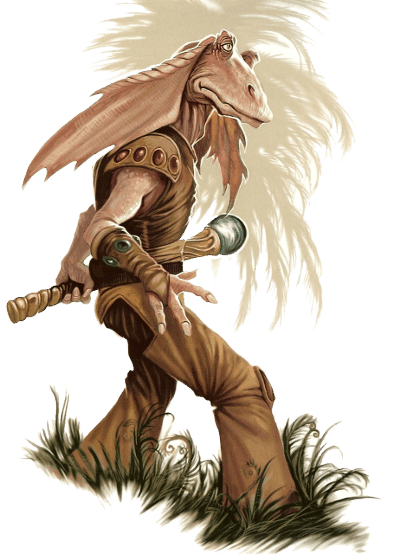
\includegraphics[width=6cm]{img/races/gungan.png}
\vspace{-12\baselineskip}

\begin{flushright}
\begin{tabular}{ l l }
	\textbf{Type} 			& Amphibien \\
   	\textbf{Planète} 		& Naboo \\
   	\textbf{Language} 		& Gunganese \\
   	\textbf{Orientation} 	& Lumineux \\
\end{tabular}
\end{flushright}


\vspace{7\baselineskip}

Natifs de la planète Naboo, les Gungans vivent dans des cités sous-marines, évitant autant qu'ils le peuvent la race peuplant la surface : les Humains de Naboo. 

La physiologie d'un Gungan est de type humanoïde, quoique plus grand et plus fin qu'un Humain. Les Gungans possèdent de longues oreilles tombantes, des narines souples et des membranes rétractiles protégeant les yeux lors de leur déplacement aquatique. Leurs articulations sont libres et les ligaments très souples, permettant aux amphibiens de nager avec aisance sous l'eau.

La culture Gungan est une relation poussée entre la nature et l'individu. Ils essaient de ne pas utiliser la technologie.

\begin{description}[align=left]
\item [Aquatique] 			% CAP +2 +1
		Les gungans vivent dans les grandes étendues d'eau de Naboo, ils ne peuvent se noyer. Ils se déplace sous l'eau beacoup plus vite que n'importe qu'elle autre espèce.\\
		\emph{d6 Natation}\\
		\emph{Allure sous l'eau = d Natation}
\item [Mollusque] 			% CAP +3
		Leurs articulations sont libres et les ligaments très souples, permettant aux amphibiens de nager avec aisance sous l'eau. Cette souplesse leur permet de se faufiler dans des endroits étroits et d'esquiver les attaques avec plus de réussite.\\
		\emph{Esquive}
\end{description}